% This is an English UHH LaTeX  template for a report or student assignment that is
% built on the  'ireport' R package.

% -------------------------------
% --- PREAMBLE ---
% -------------------------------

% Options for packages loaded elsewhere {{{
\PassOptionsToPackage{unicode}{hyperref}
\PassOptionsToPackage{hyphens}{url}
% }}}


% Define document type (here article) {{{
\documentclass[
11pt,
a4paper]{article}
% }}}


% Coding, Language {{{
% }}}


% Packages {{{
\usepackage{amssymb,amsmath}  	% for math symbols and equations
\usepackage{array}				% extends the array and tabular environments
\usepackage{booktabs}			% for publication quality tables in LaTeX
\usepackage{calc}				% for simple arithmetic in LaTeX commands
\usepackage{eso-pic}			% to add picture commands (or backgrounds) to every page.
\usepackage{fancyhdr}			% for constructing headers and footers
\usepackage{fontspec}			% allows loading of OpenType fonts in a LATEX document
\usepackage{hyperref}			% to handle cross-referencing commands in LaTeX
\usepackage{lastpage}			% allows reference to last page
\usepackage{longtable}			% handles multipage tables
\usepackage{moreverb}			% extends the verbatim package
\usepackage{multirow}			% creates tabular cells spanning multiple rows
\usepackage{natbib}				% flexible bibliography support
\usepackage{tabularx} 			% defines an environment tabularx, an extension of tabular
\usepackage{tikz}				% tool to create graphic elements in LaTeX
\usepackage{titlesec}			% interface to sectioning commands
\usepackage{url}				% verbatim with URL-sensitive line breaks
\usepackage{xcolor}				% extends LATEX's color facilities
\usepackage{colortbl}			% to add colour to LaTeX tables
\usepackage{enumitem}     % to adjusted itemized and enumerated lists
% }}}


% Define Layout {{{
\usepackage{geometry}			% user interface to customize page layout
 \geometry{
 left=25mm,
 right=25mm,
 top=12mm,
 bottom=20mm,
 includeheadfoot,
 }
% }}}


% Graphics {{{
\usepackage{graphicx}
\graphicspath{ {images/} } % images have to be in the /image subfolder
\makeatletter
\def\maxwidth{\ifdim\Gin@nat@width>\linewidth\linewidth\else\Gin@nat@width\fi}
\def\maxheight{\ifdim\Gin@nat@height>\textheight\textheight\else\Gin@nat@height\fi}
\makeatother
% Scale images if necessary, so that they will not overflow the page
% margins by default, and it is still possible to overwrite the defaults
% using explicit options in \includegraphics[width, height, ...]{}
\setkeys{Gin}{width=\maxwidth,height=\maxheight,keepaspectratio}
% }}}


% Define position of graphics
\usepackage{float} % to place the float at precisely the location in the LaTeX code
\floatplacement{figure}{H}
\floatplacement{table}{H}
% }}}


% Define colors for hyperlinks: {{{
\definecolor{linkcol}{HTML}{0271BB} %darkblue (027BCB)
\definecolor{filecol}{HTML}{b70000} %darkred (b70000)
\definecolor{urlcol}{HTML}{b70000} %darkred (b70000)
\definecolor{citecol}{HTML}{0271BB} %darkblue (027BCB)
% }}}


% Hypersetup {{{
\hypersetup{
colorlinks=true,
linkcolor=linkcol,
filecolor=filecol,
urlcolor=urlcol,
citecolor=citecol,
bookmarks=true,
linktocpage=true,
pdfpagemode=UseOutlines,
}
% }}}


\urlstyle{same} % disable monospaced font for URLs




% Modify lists: {{{
\setlist[itemize]{noitemsep, topsep=1pt}
\setlist[enumerate]{noitemsep, topsep=1pt}
% }}}


% to allow syntax highlighting:


\usepackage[normalem]{ulem}
% Avoid problems with \sout in headers with hyperref
\pdfstringdefDisableCommands{\renewcommand{\sout}{}}

\setlength{\emergencystretch}{3em} % prevent overfull lines
\providecommand{\tightlist}{%
  \setlength{\itemsep}{0pt}\setlength{\parskip}{0pt}}


\setcounter{secnumdepth}{5}




% Name definitions  {{{
% Definition of pagename (so it can be changed by user
\newcommand\pagename{Page}
% }}}



% Text formatting  {{{

% Fonts
\defaultfontfeatures{Mapping = tex-text}
\setmainfont[BoldFont = font_bold.ttf, ItalicFont = font_italic.ttf, BoldItalicFont = font_bolditalic.ttf]{font_regular.ttf}
\newfontfamily\headingfont[ItalicFont = font_bolditalic.ttf]{font_bold.ttf}

% setting caption text
\usepackage[font=small,labelfont=bf]{caption}

% Paragraph settings
\setlength{\parindent}{0em}           %  indentation at the first line of a paragraph (here set to 0)
\setlength{\parskip}{0.5em}             % paragraph spacing
\renewcommand{\baselinestretch}{1.0}    % line spacing (here single)

% Custom colors for headers
\definecolor{bluegray}{HTML}{3B515B} 
\definecolor{blue}{HTML}{0271BB} 

% change font size and colors of section headers: 
\titleformat*{\section}{\Large\bfseries\color{blue}}
\titleformat*{\subsection}{\large\bfseries\color{bluegray}}
\titleformat*{\subsubsection}{\large\bfseries\color{bluegray}}

% setting head hight
\setlength{\headheight}{13.59999pt}

% }}}


% Settings specified by user

  \usepackage{booktabs}
  \usepackage{longtable}
  \usepackage{array}
  \usepackage{multirow}
  \usepackage{wrapfig}
  \usepackage{float}
  \usepackage{colortbl}
  \usepackage{pdflscape}
  \usepackage{tabu}
  \usepackage{threeparttable}
  \usepackage{threeparttablex}
  \usepackage[normalem]{ulem}
  \usepackage{makecell}
  \usepackage{xcolor}



%%%%%%%%%%%%%%%%%%%%%%%%%%%%%%%%%%%%%%%%%%%%%


% Title
\title{Document title}
\date{\today}

\makeatletter
\renewcommand{\maketitle}{\bgroup\setlength{\parindent}{0pt}
\begin{flushleft}
  \textbf{\color{bluegray}\huge\@title}
  \vskip 0.25em%
    \textbf{\color{bluegray}\large Subtitle}
  
  \vskip 0.5em%
    \large\color{bluegray} Author name(s)\par
    \color{bluegray}\@date
\end{flushleft}\egroup
}
\makeatother


% Header and footer {{{
\pagestyle{fancy}

\thispagestyle{empty}

  \fancyhead[L]{Runninghead}
 
  \fancyhead[R]{Author}
 

% }}}


% Adjust abstract section (full width and left aligned)
\renewenvironment{abstract}
 {\small
  \begin{flushleft}
  \bfseries \abstractname\vspace{-0.5em}\vspace{0pt}
  \end{flushleft}
  \list{}{
    \setlength{\leftmargin}{.0cm}
    \setlength{\rightmargin}{\leftmargin}
  }
  \item\relax}
 {\endlist}



% Document ----------------

\begin{document}

\maketitle

\begin{abstract}
Lorem ipsum dolor sit amet, consectetur adipiscing elit. Aenean ut elit
odio. Donec fermentum tellus neque, vitae fringilla orci pretium vitae.
Fusce maximus finibus facilisis. Donec ut ullamcorper turpis. Donec ut
porta ipsum. Nullam cursus mauris a sapien ornare pulvinar. Aenean
malesuada molestie erat quis mattis. Praesent scelerisque posuere
faucibus. Praesent nunc nulla, ullamcorper ut ullamcorper sed, molestie
ut est. Donec consequat libero nisi, non semper velit vulputate et.
Quisque eleifend tincidunt ligula, bibendum finibus massa cursus eget.
Curabitur aliquet vehicula quam non pulvinar. Aliquam facilisis tortor
nec purus finibus, sit amet elementum eros sodales. Ut porta porttitor
vestibulum.
\end{abstract}




\hypertarget{introduction}{%
\section{Introduction}\label{introduction}}

Configure the YAML header including the following elements:

\begin{itemize}
\tightlist
\item
  \texttt{title}: Title
\item
  \texttt{subtitle}: Subitle; remove option completely, if you don't
  need a subtitle.
\item
  \texttt{author}: Character of single or multiple author(s)
\item
  \texttt{header\_left}: A running title as left header; remove option
  to leave blank.
\item
  \texttt{header\_right}: A second right header (e.g.~authors); remove
  option to leave blank.
\item
  \texttt{date}: The date; by default \texttt{\textbackslash{}date},
  will populate the date automatically.
\item
  \texttt{fontsize}: Font size for body text; choose between
  \texttt{10pt}, \texttt{11pt} (default), and \texttt{12pt}.
\item
  \texttt{linkcolor}, \texttt{filecolor}, \texttt{citecolor},
  \texttt{urlcolor}: Specify here colors for internal links, external
  links, citation links, and linked URLs, respectively, if you don't
  want the default colors; use options allowed by xcolor, including the
  dvipsnames, svgnames, and x11names lists.
\item
  \texttt{german}: If option is set to \texttt{true}, the table and
  figure caption as well as the abstract and reference header will be in
  German; default is \texttt{false} (i.e., English).
\item
  \texttt{bibliography}: A path to the bibliography file(s) to use for
  references (BibTeX \emph{.bib} file). This template uses the
  bibliography-related package
  \href{https://ctan.org/pkg/natbib}{natbib}. The current file
  `references.bib' in the `bib/' folder includes 3 dummy references;
  either insert your references into this file or replace the file with
  your own.
\item
  \texttt{bibliographystyle}: The style is provided in the bibstyle.bst
  file, which adopts the
  \href{https://uk.sagepub.com/sites/default/files/sage_harvard_reference_style_0.pdf}{SAGE
  Harvard} reference style. Just leave the file as it is.
\item
  \texttt{abstract}: Write here your abstract or remove option if you
  don't want to include an abstract.
\item
  \texttt{output}: The nested fields for the output field are based on
  the arguments of the output function. Since
  \texttt{UHHformats::pdf\_simple} is based on
  \texttt{rmarkdown::pdf\_document}, see its help page for more options.
  Current default settings are

  \begin{itemize}
  \tightlist
  \item
    \texttt{number\_sections:\ TRUE}
  \item
    \texttt{highlight:\ "kate"}
  \item
    \texttt{font\ =\ "Helvetica"}
  \item
    \texttt{citation\_package:\ "natbib"}
  \item
    \texttt{latex\_engine:\ "xelatex"}
  \end{itemize}
\item
  \texttt{header\_includes}: Here you can add additional \LaTeX code to
  include in the header, before the
  \texttt{\textbackslash{}\textbackslash{}begin\textbackslash{}\{document\textbackslash{}\}}
  statement.
\item
  If you want to add additional LaTeX code to include before the
  \texttt{\textbackslash{}\textbackslash{}end\textbackslash{}\{document\textbackslash{}\}}
  statement use the field \texttt{include\_after}.
\end{itemize}

If you are associated with the UHH you can also use the University's own
font ``TheSansUHH''. In that case replace \texttt{font\ =\ "Helvetica"}
with \texttt{font\ =\ "TheSansUHH"}. To use another font, simply use the
setting ``other'' and replace the `font\_XXX.ttf' files in the working
directory with your own files. Please note, that you have to name these
files exactly as the template font files.

\hypertarget{methods}{%
\section{Methods}\label{methods}}

\hypertarget{r-markdown-syntax-vs-syntax}{%
\subsection{\texorpdfstring{R Markdown syntax vs
\LaTeX syntax}{R Markdown syntax vs syntax}}\label{r-markdown-syntax-vs-syntax}}

As with any .Rmd file you can write the entire report in the R Markdown
syntax. However, if you are familiar with \LaTeX you can also mix both:

\hypertarget{r-markdown-subsection}{%
\subsubsection{R Markdown subsection}\label{r-markdown-subsection}}

This is a dummy text to show you how to write in \textbf{bold} and in
\emph{italics}.

\subsubsection{LaTeX subsection}

This is a dummy text to show you that you can also write in
\textbf{bold} and in \textit{italics} with \LaTeX.

\hypertarget{cross-referencing-within-the-report}{%
\subsection{Cross-referencing within the
report}\label{cross-referencing-within-the-report}}

To cross-references figures or tables you have to have a:

\begin{itemize}
\tightlist
\item
  \textbf{caption to your figure (or table)}:

  \begin{itemize}
  \tightlist
  \item
    NOTE: figures without a caption will be included directly as images
    and will therefore not be a numbered figure
  \end{itemize}
\item
  \textbf{labeled code chunk}: this provides the identifier for
  referencing the figure or table generated by the chunk.
\end{itemize}

Cross-references within the text can then be made using the standard
\LaTeX syntax \texttt{\textbackslash{}@ref\{type:label\}}, where label
is the chunk label and type is the environment being referenced
(e.g.~tab, fig, or eq). Examples are given in the sections below
(e.g.~in \protect\hyperlink{r-markdown-table}{R Markdown table}).

To cross-reference sections simply put the section header in square
brackets, e.g.~\protect\hyperlink{r-output}{R output} via
\texttt{{[}R\ output{]}}.

\hypertarget{mathematics}{%
\subsection{Mathematics}\label{mathematics}}

Use mathematics as usual with the dollar sign \texttt{\$}; either in
inline mode with one dollar sign, e.g.~\(E = mc^2\), or in display mode
with two:

\[E = mc^2\]

Important to note: do not leave a space between the \texttt{\$} and your
mathematical notation.

Alternatively, you can use \LaTeX for more control, e.g.~for setting
equation numbers that can be cross-referenced:

\begin{equation} \label{eq:mean}
  \bar{X} = \frac{\sum_{i=1}^n X_i}{n}
\end{equation}

You may refer to this equation using
\texttt{\textbackslash{}ref\{eq:label\}}, e.g., see Equation
\ref{eq:mean}

\newpage

\hypertarget{results}{%
\section{Results}\label{results}}

\hypertarget{r-output}{%
\subsection{R output}\label{r-output}}

R output is typically shown in the monospace font (here an example with
the \texttt{mtcars} dataset in the subfolder \texttt{data/}):

\begin{verbatim}
##       mpg             cyl             disp             hp       
##  Min.   :10.40   Min.   :4.000   Min.   : 71.1   Min.   : 52.0  
##  1st Qu.:15.43   1st Qu.:4.000   1st Qu.:120.8   1st Qu.: 96.5  
##  Median :19.20   Median :6.000   Median :196.3   Median :123.0  
##  Mean   :20.09   Mean   :6.188   Mean   :230.7   Mean   :146.7  
##  3rd Qu.:22.80   3rd Qu.:8.000   3rd Qu.:326.0   3rd Qu.:180.0  
##  Max.   :33.90   Max.   :8.000   Max.   :472.0   Max.   :335.0
\end{verbatim}

\hypertarget{tables}{%
\subsection{Tables}\label{tables}}

\hypertarget{r-markdown-table}{%
\subsubsection{R Markdown table}\label{r-markdown-table}}

Table \ref{tab:rmd_tab} is a R Markdown table including a caption (note:
the table number is automatically assigned) and label for
cross-referencing:

\begin{longtable}[]{@{}lcr@{}}
\caption{Your Caption \label{tab:rmd_tab}}\tabularnewline
\toprule\noalign{}
A & New & Table \\
\midrule\noalign{}
\endfirsthead
\toprule\noalign{}
A & New & Table \\
\midrule\noalign{}
\endhead
\bottomrule\noalign{}
\endlastfoot
left-aligned & center-aligned & right-aligned \\
\$123 & \$456 & \$789 \\
\emph{italics} & \st{strikethrough} & \textbf{boldface} \\
\end{longtable}

\hypertarget{tables-generated-with-r}{%
\subsubsection{Tables generated with R}\label{tables-generated-with-r}}

\hypertarget{using-the-knitr-and-kableextra-packages}{%
\paragraph{\texorpdfstring{Using the \emph{knitr} and \emph{kableExtra}
packages}{Using the knitr and kableExtra packages}}\label{using-the-knitr-and-kableextra-packages}}

Table \ref{tab:kable_tab} is an example when using
\texttt{knitr::kable()} to generate the table and \emph{kableExtra}
functions to modify it:

\begin{table}

\caption{\label{tab:kable_tab}A table produced with knitr and kableextra}
\centering
\fontsize{9}{11}\selectfont
\begin{tabular}[t]{lrrrrrr}
\toprule
\multicolumn{1}{c}{\textbf{ }} & \multicolumn{4}{c}{\textbf{Group 5}} & \multicolumn{2}{c}{\textbf{Group 6}} \\
\cmidrule(l{3pt}r{3pt}){2-5} \cmidrule(l{3pt}r{3pt}){6-7}
\multicolumn{1}{c}{ } & \multicolumn{2}{c}{Group 1} & \multicolumn{2}{c}{Group 2} & \multicolumn{1}{c}{Group 3} & \multicolumn{1}{c}{Group 4} \\
\cmidrule(l{3pt}r{3pt}){2-3} \cmidrule(l{3pt}r{3pt}){4-5} \cmidrule(l{3pt}r{3pt}){6-6} \cmidrule(l{3pt}r{3pt}){7-7}
  & mpg & cyl & disp & hp & drat & wt\\
\midrule
\cellcolor{gray!6}{Mazda RX4} & \cellcolor{gray!6}{21.0} & \cellcolor{gray!6}{6} & \cellcolor{gray!6}{160} & \cellcolor{gray!6}{110} & \cellcolor{gray!6}{3.90} & \cellcolor{gray!6}{2.620}\\
Mazda RX4 Wag & 21.0 & 6 & 160 & 110 & 3.90 & 2.875\\
\cellcolor{gray!6}{Datsun 710} & \cellcolor{gray!6}{22.8} & \cellcolor{gray!6}{4} & \cellcolor{gray!6}{108} & \cellcolor{gray!6}{93} & \cellcolor{gray!6}{3.85} & \cellcolor{gray!6}{2.320}\\
Hornet 4 Drive & 21.4 & 6 & 258 & 110 & 3.08 & 3.215\\
\cellcolor{gray!6}{Hornet Sportabout} & \cellcolor{gray!6}{18.7} & \cellcolor{gray!6}{8} & \cellcolor{gray!6}{360} & \cellcolor{gray!6}{175} & \cellcolor{gray!6}{3.15} & \cellcolor{gray!6}{3.440}\\
\bottomrule
\multicolumn{7}{l}{\rule{0pt}{1em}\textit{Note: }}\\
\multicolumn{7}{l}{\rule{0pt}{1em}Your comments go here.}\\
\end{tabular}
\end{table}

\hypertarget{the-xtable-package}{%
\paragraph{\texorpdfstring{The \emph{xtable}
package}{The xtable package}}\label{the-xtable-package}}

Another useful package for tables for PDF output is
\href{https://cran.r-project.org/web/packages/xtable/vignettes/xtableGallery.pdf}{xtable}.
The following code will produce an example table if the \emph{xtable}
package is installed. Note that you need to add the chunk option
\texttt{results\ =\ "asis"} inside \texttt{\{r\}} otherwise the PDF will
contain the \LaTeX code of the table!

\begin{table}[ht]
\centering
\caption{A table made with xtable} 
\label{tab:xtable_tab}
\begin{tabular}{rrrrrrr}
  \toprule
 & mpg & cyl & disp & hp & drat & wt \\ 
  \midrule
Mazda RX4 & 21.00 &   6 & 160.00 & 110 & 3.90 & 2.62 \\ 
  Mazda RX4 Wag & 21.00 &   6 & 160.00 & 110 & 3.90 & 2.88 \\ 
  Datsun 710 & 22.80 &   4 & 108.00 &  93 & 3.85 & 2.32 \\ 
  Hornet 4 Drive & 21.40 &   6 & 258.00 & 110 & 3.08 & 3.21 \\ 
  Hornet Sportabout & 18.70 &   8 & 360.00 & 175 & 3.15 & 3.44 \\ 
   \bottomrule
\end{tabular}
\end{table}

\hypertarget{figures}{%
\subsection{Figures}\label{figures}}

\begin{figure}
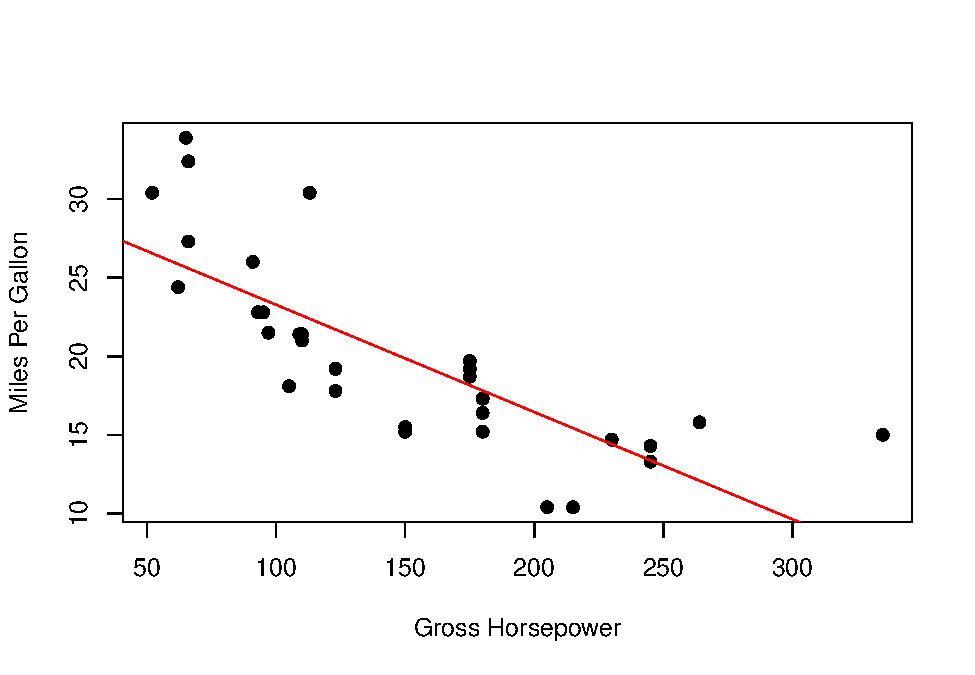
\includegraphics[width=1\linewidth]{figs/unnamed-chunk-4-1} \caption{Relationship between horsepower and fuel economy\label{fig:base-ref}}\label{fig:unnamed-chunk-4}
\end{figure}

Figures are supported from R code and can be referenced (see Figure
\ref{fig:base-ref}) by including the
\texttt{\textbackslash{}\textbackslash{}label\{\}} tag in the
\texttt{fig.cap} attribute of the R chunk:
\texttt{fig.cap\ =\ "Relationship\ between\ horsepower\ and\ fuel\ economy\textbackslash{}\textbackslash{}label\{fig:base-ref\}"}.
It is a quirky hack at the moment, see
\href{https://github.com/yihui/knitr/issues/323}{here}.

Figure \ref{fig:boxplot-ref} shows a boxplot with just half the width
and centered:

\begin{figure}

{\centering 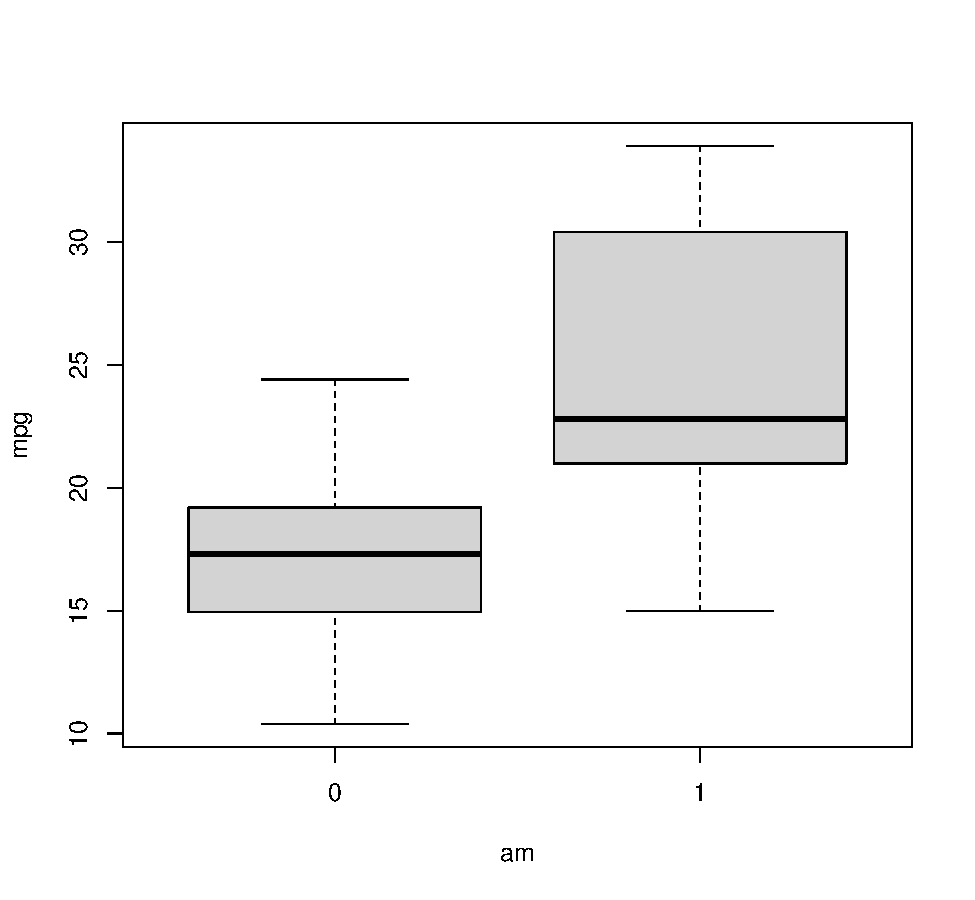
\includegraphics[width=0.5\linewidth]{figs/unnamed-chunk-5-1} 

}

\caption{Fuel differences between transmission types (0 = automatic, 1 = manual)\label{fig:boxplot-ref}}\label{fig:unnamed-chunk-5}
\end{figure}

\hypertarget{discussion}{%
\section{Discussion}\label{discussion}}

Lorem ipsum dolor sit amet, consetetur sadipscing elitr, sed diam nonumy
eirmod tempor invidunt ut labore et dolore magna aliquyam erat, sed diam
voluptua. At vero eos et accusam et justo duo dolores et ea rebum. Stet
clita kasd gubergren, no sea takimata sanctus est Lorem ipsum dolor sit
amet. Lorem ipsum dolor sit amet, consetetur sadipscing elitr, sed diam
nonumy eirmod tempor invidunt ut labore et dolore magna aliquyam erat,
sed diam voluptua. At vero eos et accusam et justo duo dolores et ea
rebum. Stet clita kasd gubergren, no sea takimata sanctus est Lorem
ipsum dolor sit amet. Lorem ipsum dolor sit amet, consetetur sadipscing
elitr, sed diam nonumy eirmod tempor invidunt ut labore et dolore magna
aliquyam erat, sed diam voluptua. At vero eos et accusam et justo duo
dolores et ea rebum. Stet clita kasd gubergren, no sea takimata sanctus
est Lorem ipsum dolor sit amet.

\hypertarget{adding-citations-and-bibliography}{%
\section{Adding citations and
bibliography}\label{adding-citations-and-bibliography}}

Link a \texttt{.bib} document via the YAML header and the bibliography
will be printed at the very end (as usual). The default bibliography
style is provided in the \texttt{bib.bst} file (do not delete), which
adopts the
\href{https://uk.sagepub.com/sites/default/files/sage_harvard_reference_style_0.pdf}{SAGE
Harvard} reference style.

References can be cited directly within the document using the R
Markdown equivalent of the \LaTeX citation system \texttt{{[}@key{]}},
where key is the citation key in the first line of the entry in the .bib
file. Example: \citep{Taylor1937}. To cite multiple entries, separate
the keys by semicolons (e.g., \citep{Knupp1999, Kamm2000}.

There is also the package \href{https://github.com/crsh/citr}{citr},
which I highly recommend: \emph{citr} provides functions and an RStudio
add-in to search a BibTeX-file to create and insert formatted Markdown
citations into the current document. If you are using the reference
manager \href{https://www.zotero.org/}{Zotero} the add-in can access
your reference database directly.

\hypertarget{software}{%
\subsection{Software}\label{software}}

If you want to include a paragraph on the software used, here is some
example text/code to get the current R and package versions. The code to
create a separate bibliography file named `packages.bib' with all
package references has already been added at the beginning of this
script (code chunk `generate-package-refs').

All analyses were performed using the statistical software R (version
4.3.0) \citep{R-base}. This report, including tables and figures, was
generated using the packages `rmarkdown' (version 2.23)
\citep{R-rmarkdown}, `bookdown' (version 0.34) \citep{R-bookdown},
`UHHformats' (version 1.0.0.9000) \citep{R-UHHformats}, `knitr' (version
1.43) \citep{R-knitr}, `kableExtra' (version 1.3.4)
\citep{R-kableExtra}, `xtable' (version 1.8.4) \citep{R-xtable}, and
`tidyverse' (version 2.0.0) \citep{R-tidyverse}

\clearpage

  \bibliographystyle{bib/bibstyle.bst}
  \bibliography{bib/references.bib, bib/packages.bib}




\end{document}
